%%
%% This is file `mcmthesis-demo.tex',
%% generated with the docstrip utility.
%%
%% The original source files were:
%%
%% mcmthesis.dtx  (with options: `demo')
%% 
%% -----------------------------------
%% 
%% This is a generated file.
%% 
%% Copyright (C)
%%     2010 -- 2015    by Zhaoli Wang
%%     2014 -- present by Liam Huang
%% 
%% This work may be distributed and/or modified under the
%% conditions of the LaTeX Project Public License, either version 1.3
%% of this license or (at your option) any later version.
%% The latest version of this license is in
%%   http://www.latex-project.org/lppl.txt
%% and version 1.3 or later is part of all distributions of LaTeX
%% version 2005/12/01 or later.
%% 
%% This work has the LPPL maintenance status `maintained'.
%% 
%% The Current Maintainer of this work is Liam Huang.
%% 
\documentclass{mcmthesis}
\mcmsetup{CTeX = false,   % 使用 CTeX 套装时,设置为 true
        tcn = 2001560, problem = C,
        sheet = true, titleinsheet = true, keywordsinsheet = false,
        titlepage = false, abstract = true}
\usepackage{palatino}
\usepackage{lipsum}

% \title{A Wealth of Data}
% \author{\small \href{http://www.latexstudio.net/}
%   {
\includegraphics[width=7cm]{mcmthesis-logo}}}
\date{\today}

\usepackage{geometry}
\geometry{left=1in,right=0.75in,top=1in,bottom=1in}
\usepackage{lastpage}

%%%%%%%%%%%%%%%%%%%%%%%%%%%%%%%%%%%%%%%%
\newcommand{\Problem}{C}    % 换成你的题号
\newcommand{\Team}{2001560} % 换成你的队号
%%%%%%%%%%%%%%%%%%%%%%%%%%%%%%%%%%%%%%%%

\begin{document}

\thispagestyle{empty}
\vspace*{-16ex}
\centerline{\begin{tabular}{*3{c}}
	\parbox[t]{0.3\linewidth}{\begin{center}\textbf{Problem Chosen}\\ \Large \textcolor{red}{\Problem}\end{center}}
	& \parbox[t]{0.3\linewidth}{\begin{center}\textbf{2020\\ MCM/ICM\\ Summary Sheet}\end{center}}
	& \parbox[t]{0.3\linewidth}{\begin{center}\textbf{Team Control Number}\\ \Large \textcolor{red}{\Team}\end{center}}	\\
	\hline
\end{tabular}}
%%%%%%%%%%% Begin Summary %%%%%%%%%%%

\vspace{2em}
\begin{center}
\Large\bf Look Beyond The Data   % 论文标题
\end{center}

In online shopping platforms, such as Amazon, customers can post reviews to express their satisfaction with the product. These reviews can be used as a reference or other users when purchasing. They can also be analyzed and organized by the company as an essential basis for formulating sales strategies, improving products, or analyzing sales conditions. To help companies achieve this goal, we have designed and built relevant models for extracting useful information about market operations from product ratings and reviews.

To make the results as accurate and credible as possible, we think that a review (including star rating and text content) can be considered from the following two aspects: 1) review content; 2) review quality. The content of the review should comprehensively consider the rating and the text review, to reduce misleading caused by misoperation or fake rating. To quantify the text content, we used the analysis method of word frequency statistics. For the quality of reviews, we comprehensively consider four factors: the length of the review, whether Vine, helpfulness votes, and the departure between stars and reviews to find more reliable reviews and assign higher weight to them in the analysis.

Based on this model, the customer's overall evaluation of the product over a period of time can be regarded as the reputation of the product. We examine the changing trend of product reviews in the time dimension to obtain the change of the reputation of the product in the market, and by looking for and analyzing the turning point of this trend, we can predict the success of the product. Besides, by using the TF-IDF method to build an LDA model of the review content and analyze it, we also found that certain specific words are closely related to the rating level.
We believe that our model can, to a certain extent, obtain the market's actual evaluation of the product from the reviews promptly. But this model has some disadvantages. Due to a lack of data, some parameters in the module were roughly determined through common sense or trial. If there is more data supported, our model may be more accurate.

%%%%%%%%%%% End Summary %%%%%%%%%%%

\clearpage
\pagestyle{fancy}
% Uncomment the next line to generate a Table of Contents
%\tableofcontents 
\newpage
\setcounter{page}{1}
\rhead{Page \thepage\ of \pageref{LastPage}}

\tableofcontents
\newpage

% \begin{abstract}
%   \lipsum[1]
% \end{abstract}
% \maketitle
%%
%% Generate the Memorandum, if it's needed.
\memoto{Marketing Director of Sunshine Company}
\memofrom{MCM Team \#2001560}
\memosubject{Special Online Sales Strategy for Sunshine Company}
\memodate{March 9, 2020}
% \logo{\LARGE I'm pretending to be a LOGO!}
\begin{memo}[Letter]
Dear Marketing Director,
\\\\
Thank you for your trust in our team. We have learned that you want to start with ratings and reviews and get some relevant parameters or metrics to quantify the reputation of the product, thereby increasing product attractiveness and sales. After a thorough study, we have built a model that analyze the synthesize evaluation of products to help you identify the reputation of the products and whether they are successful in the online market.
\\\\
After analyzing the data, we found that we cannot evaluate the quality and reputation of a product based on star ratings only. Because not only the star rating and the content of the review do not match well, there are some cases where non-purchasers make biased reviews of the product. These problematic stars and reviews can mislead customers, affect their shopping decisions, affect future review trends, and even damage product reputation.
\\\\
Firstly, we removed reviews from non-purchasers(Amazon Vine members are identified as purchasers) from the data, which minimizes the potential for malicious reviewers to damage the reputation of the product. 
\\\\
Then, we studied each review through TD-IDF (information retrieval and data mining technology) to analyze the term frequency and give each review a sentiment score, which indicates the actual semantics. By coefficient simulation, We found that there has a strong correlation between the stars and sentiment score while some are not fitting well, which shows that star rating and sentiment score both modify the quality of the product.
\\\\
We suppose there is a distinction between product reputation and product quality for various quality reviews can have diverse effects on product reputation. A single word 'Perfect' is inadequate, while a detailed description of the praise brings more forward message to the customer. Amazon Vine member reviews and reviews with high ratings are credible.We established a review quality score model to value the review. When the star rating and the sentiment score are similar, the quality is more top; when the star rating and the review sentiment score do not harmonize, the quality is lower.
\\\\
By synthesize evaluation model, we take word length, helpfulness rate, whether it is from a vine member and review quality score and sentiment score into consideration to define the synthesize evaluation score, which represents a product's reputation.
\\\\
When your products are on the online market, by examining the synthesize evaluation score over time, you can discern whether the products are potentially fruitful. Through analyzing the three types of products' synthesize evaluation score, we list several reasons for the changes in product reputation in a certain period. They assists you to pay attention to some particular breakpoints to optimize listing in time and improve the product reputation.
\begin{itemize}
	\item A specific review may incite customers to write positive or negative reviews. You need to have an eye on negative reviews and appropriately invite customers to write reviews that benefit the product reputation.

	\item Poor overall review quality (inconsistent star ratings and review content) may cause product reputation to decline.

	\item Inviting more Amazon Vine Members to write reviews can improve the product reputation.

	\item When multiple bad reviews with high quality appear, not only estimating the negative impact of these reviews is necessary, but also pay attention to the shortcomings of products, and feedback these opinions to the design manufacturers to improve the products.
\end{itemize}
We sincerely hope that it will provide you with useful information. Wish very best wished for your job and your products!\\\\
Team \#2001560

\end{memo}

\section{Introduction}
\subsection{Background}
In recent years, quantities of customers prefer shopping online for its less spacetime limitation and the convenient home delivery service. However, compared to the traditional physical stores, customers can only evaluate products by the provided profile and pictures instead of seeing or testing the real ones. The information gap here is one of the leading causes of dissatisfied purchases. To help customers know the product better, many online marketplace platforms, such as Amazon, launch a "review system". Customers can express their level of satisfaction and further opinions or information about purchases through rating and reviewing. That additional information can help not only other customers make purchasing decisions, but companies improve the pros and cons of product design.

However, we found that not all reviews are equally relevant. Some reviews are too general; some people's ratings do not match their reviews; there are even deliberately misleading reviews, such as malicious defamation from competitors or the raise by the bribed reviewers. Therefore, when using data to assist business decisions, we need to analyze data carefully and comprehensively to obtain more accurate results. More factors should be considered, such as the ratings, review contents, and review time, rather than straightly calculate the average rating level.

\subsection{Problem Restatement}
Analyze the three product data sets to describe quantitative and/or qualitative patterns, relationships that help evaluate a product's star ratings, reviews, and helpfulness ratings. Use data to demonstrate that they are valuable.

Solve the following issues through modeling:
\begin{itemize}
  \item Determine the most informative metric based on ratings and reviews. This metric can track the product ratings of three products when they are on the market.
  
  \item Analyze the relationship between product ratings and time in three data sets.
  
  \item Look for critical factors that can affect the inflection point of product ratings through time.
  
  \item Analyze whether there will be more a series of positive or negative reviews over a while and whether customer star ratings will be affected by recent reviews.
  
  \item Whether star rating and the keyword of review content match.
\end{itemize}

\subsection{Data}
\subsubsection{Data Source}
Our model is informed by the customer-supplied ratings and reviews for microwave ovens, baby pacifiers, and hair dryers sold in the Amazon marketplace over more than ten years.
\subsubsection{Data Pre-processing}
We did the following to sanitize the data set:
\begin{itemize}
  \item Remove factors that were not measured at all, such as marketplace and product category, for they can not present any information.
  
  \item Remove the redundant factors, such as review\_id and product\_id, for they can be completely replaced by customer\_id and product\_parent.
  
  \item Remove factors that could mislead the model, such as verify\_purchase==N while vine==N.
  
  \item Remove some garbled character.
\end{itemize}

We remove the reviews which have not been verified because we consider that reviews from those who have not bought the product are unreliable. Besides, we find that those people commit a more low rating (1 star or two stars) than those are verified purchases. We speculate that slander from competitors may be one of the reasons for this phenomenon.

\begin{figure}[h]
  \small
  \centering
  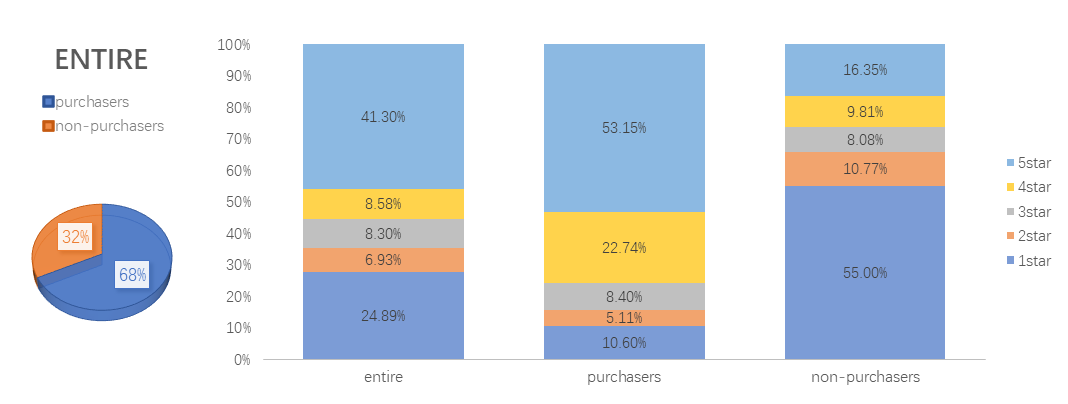
\includegraphics[width=12cm]{notbuy-micro.png}
  \caption{ratings for the microwave}
\end{figure}

\begin{figure}[h]
  \small
  \centering
  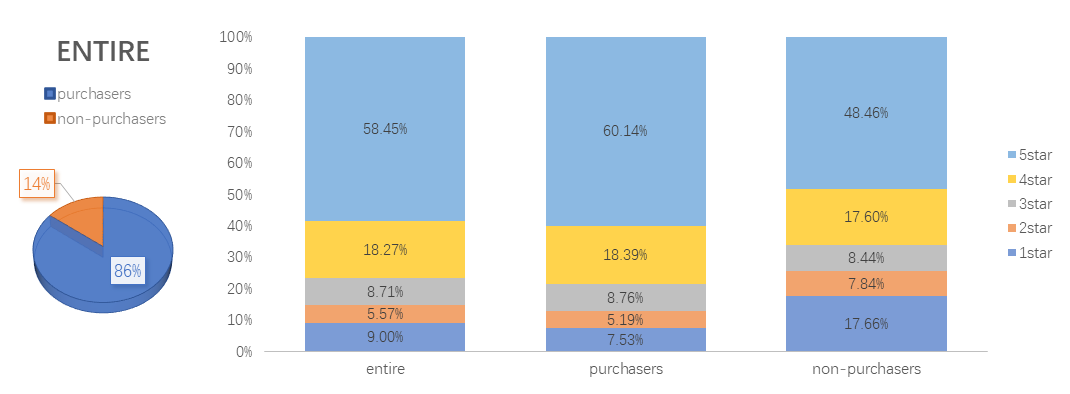
\includegraphics[width=12cm]{notbuy-dryer.png}
  \caption{ratings for the hair-dryer}
\end{figure}

\section{Assumptions}
\begin{itemize}
  \item Merchant's purpose: Guide users to buy products with quality reviews and recent reviews.
\end{itemize}
\begin{itemize}
  \item The content of the review and the star rating should be the same. People believe in reviews when review content is inconsistent with star ratings.

Reason: Based on popular psychology, real language is convincing 
\end{itemize}
\begin{itemize}
  \item Amazon Vine members' reviews are credible, excluding subjective factors that give high ratings for free products.

Reason: Big data select Amazon Vine members. Their evaluations are more objective and practical.
\end{itemize}
\begin{itemize}
  \item Actual purchasers' reviews are credible.

Reason: People who have already experienced the product know more about the actual performance of the product.
\end{itemize}
\begin{itemize}
  \item Comments from actual non-purchasers (except Amazon Vine members) are untrustworthy.

Reason: Amazon provides Amazon Vine members with free copies of the product. Hence Amazon Vine members should be identified as purchasers. We listed the distribution of 1-5 stars between the non-purchasers and the purchasers. It shows that the non-purchasers give more 1 star than purchasers, which may mislead the reviews.
\end{itemize}
\begin{itemize}
  \item The impact of the same purchaser on reviews is not taken into consideration; that is, each evaluation behaviour of the purchaser is independent and not related to the previous reviews.
\end{itemize}
\begin{figure}[h]
  \small
  \centering
  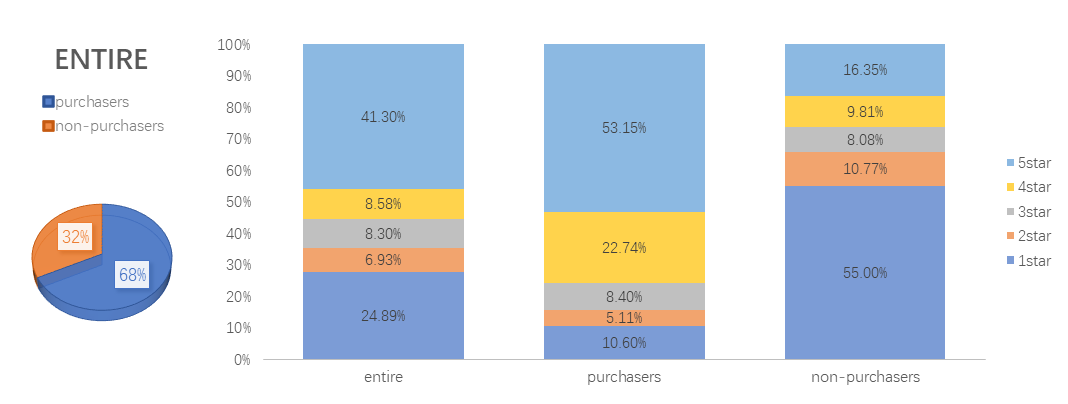
\includegraphics[width=12cm]{notbuy-micro.png}
  \caption{ratings for the microwave}
\end{figure}

\begin{figure}[h]
  \small
  \centering
  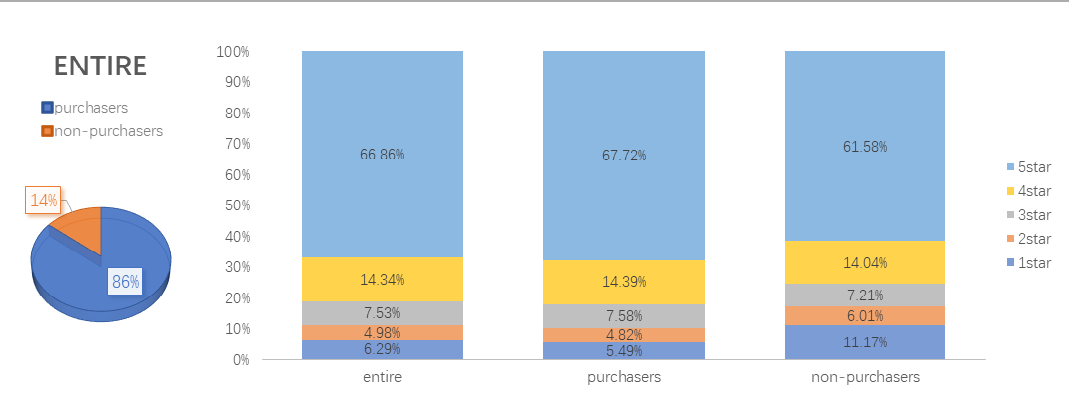
\includegraphics[width=12cm]{notbuy-per.png}
  \caption{ratings for the pacifier}
\end{figure}

\begin{figure}[h]
  \small
  \centering
  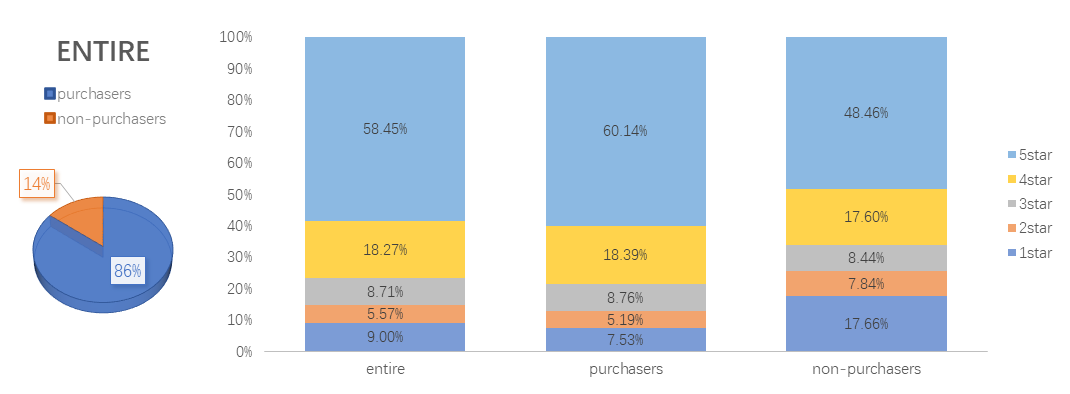
\includegraphics[width=12cm]{notbuy-dryer.png}
  \caption{ratings for the hair-dryer}
\end{figure}

\newpage
\section{Nomenclature}
\begin{table}[h]
  \centering
  \begin{tabular}{ccc}
    \hline
    Symbol & Definition\\
    \hline
    star$_{i}$ & star rating of a review i\\
    
    ER$_{i}$ & emtional rating of a review i\\
      
    d$_{i}$ & the variance between star rating and emtional rating of a review i\\

    L$_{i}$ & length of a review i\\

    Vm$_{i}$ & whether a review i is from an Amazon vine member\\
      
    Vr$_{i}$ & votes rating of a review i\\
      
    M$_{i}$ & rating of a review i\\

    Q$_{i}$ & quality of a review i\\
          
    R$_{i}$ & synthesize evaluation of a review i\\
    
    R & average review synthesize evaluation\\
      
    t & time\\
    \hline
  \end{tabular}
  \caption{variables and functions}
\end{table}

\section{Model Design}
\subsection{Review content measure}
When a user evaluates a product, he will simultaneously commit a rating and a review. These two indicators together describe his satisfaction with the product. Therefore, we can consider that the positive degree of ratings and reviews posted together are highly positively correlated in general. However, for various reasons, exceptions may occur. For example, someone may give a rating that is inconsistent with his review because of an operation error; or someone may give a higher star rating because of habit or because of a bribe from the merchant, although they are not very satisfied with the product. Therefore, when analyzing the user's evaluation of the product, we think that we should consider the influence of the rating and the review comprehensively, rather than simply counting the rating.

Because reviews are in the form of text, we need to process them first, to get a quantitative measure of user satisfaction with the product toward the review context. Reviews are generally too short for analysis using the LDA model, but we found that most of the reviews have apparent keywords. Therefore, we use the statistical method instead of NLP.

\begin{enumerate}
\item Perform word frequency statistics on each rating level, respectively.
\item Calculate the probability of each word appearing in different rating
\item Filter out words that have practical meaning and have noticeable frequency differences in different ratings
\item weighted them with the probability get a "rating" corresponding to a word
\end{enumerate}

In this way, we have a word-rating dictionary. Then in each review, we mark the above keywords and find the average rating of all keyword. Finally, according to the above algorithm, we got a review's "emotional rating" ER$_{i}$.
Taking the hair-dryer as an example: the following chart show some of the data in the process.

\begin{figure}[h]
  \small
  \centering
  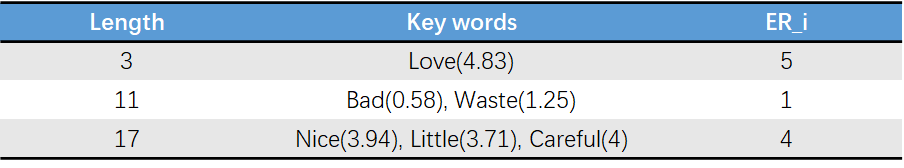
\includegraphics[width=12cm]{wordStatisticOfDryer.png}
  \caption{word statistic} \label{fig:aa}
\end{figure}

Next, we need to get a measure M$_{i}$ of a review that considers star$_{i}$ and ER$_{i}$ comprehensively.
According to our initial assumptions, if the difference between the rating and the review score is too large, it indicates that there may be some problem with this review, which can be of low reference value and should be ignored in statistics. However, from the existing data, there is not a very appropriate indicator for the measurement of the difference. Ideally, the "useful vote" of other users for reviews should be the best standard for measuring the quality and authenticity of reviews; a joint analysis can be used to find out the threshold of ignoring unreliable reviews. However, there is too little voting data for reviews in the provided data for effective analysis. 

So we decided to take another strategy. On the one hand, when posting a comment, it only takes one click to give a star rating, but a paragraph of text is required to give a review. Obviously, the former has a higher probability of misoperation. On the other hand, reviews are more informative and detailed than review stars. From life experience, in the face of a mismatch between a star rating and a review, users are more willing to believe the latter. So after a series of attempts, we finally decided to use the formula
\[
	M_{i} = 0.7 \times ER_{i} + 0.3 \times star_{i}
\]
As a measure of the content of the review.

\subsection{Review quality measure}
Using M$_{i}$, we can get a user's evaluation of the product. However, from the perspective of all reviews, each review has different reliability. In the data given, we believe that the following factors can reflect the credibility and accuracy of a review to some extent.

\subsubsection{Review votes rate}
Although the amount of helpful vote data is not enough to be a criterion for the quality of comments, we can still consider that reviews with a higher voting rate are more helpful than those with a lower one. We quantify the votes rate as follows:
\[
Vr_{i} = \begin{cases}  
\frac{helpful\_votes}{total\_votes}, & \text{if total\_votes > 0} \\
0, & \text{if total\_votes = 0}
\end{cases}
\]

\subsubsection{Length of review}
According to a study by Huang and Chen \cite{1}, the helpfulness of online review and its length has a significant positive correlation when the reviews are short enough (less than 144 words). As reviews get long, the correlation decreases. Meanwhile, the strengthening effect of review length on its helpfulness gradually decreases. Therefore, we choose to use a logarithmic function to characterize the impact of the reviews' length on its quality. Furthermore, when the length reaches a certain threshold, the review quality no longer increases. We quantify the length factor as follows:
\[
L_{i} =
\begin{cases}  
	 lg (length), &\text{if lenth of review < 100 words} \\
	2, &\text{else}
\end{cases}
\]

\subsubsection{Amazon Vine Voice}
Amazon Vine Voices are trusted users in the Amazon community for writing accurate and insightful reviews. So we can consider reviews made by them to be more accurate and reliable. The discrete variable vm$_{i}$ is used to characterize whether the customer who did this review is a Vine Voice:

\[
Vm = 
\begin{cases}  
	1, &\text{if vine = Y} \\
	0, &\text{if vine = N}
\end{cases}
\]

\subsubsection{Mismatch between ER and star}
As we discussed earlier, there may be various reasons why the text of the review does not match the star rating given. We consider these reviews to be relatively unreliable, and the degree of bias is negatively related to the credibility of the reviews. We use the following formula to quantify the impact of review mismatch with star ratings on review quality:
\[
	d_{i}  = -|ER - star|
\]

\subsubsection{Review quality measure}
After comprehensively considering the above four factors and performing experiments and adjustments on the actual data, we have the following formula for calculating the quality of reviews:
\[
Q_i = 0.2 \times Vr_i + 0.2 \times L_i + 0.2 \times vm_i + 0.1 \times d + 1
\]

\subsection{Synthesize Evaluation Model}
In summary, we got the final rating for a review:
\[
 R_i = M_i \times Q_i
\]

\section{Solution}
\subsection{Comprehensive rating}

By building a review content rating model (M$_{i}$), we can quantify a review's rating on a product. The score takes into account star ratings and review text. The following examples compare M$_{i}$ ratings, ratings, and the origin review.

\begin{table}[h]
  \centering
  \begin{tabular}{cccp{10cm}}
    \hline
    product & rate & M$_{i}$ & review\_body \\
    \hline
    microwave & 4 & 4.88 & Wonderful product. My first time using anything like this for microwave repair of burned areas. I was not sure if it would work, but to my surprise it exceeded my expections. I highly reccomend this product.\\

    pacifier & 5 & 4.35 & Bought for my new nephew and its everyone's favorite. Came on time and its just a normal pacifier with a funny saying.\\

    hair dryer & 5 & 4.76 & Excellent product!  Quick attention very well packed and fast! - It is powerful to my wife loves\\
    \hline
  \end{tabular}
  \caption{examples for M$_{i}$ rating module}
\end{table}

\subsection{Reputation of the product}

We use a comprehensive rating R to assess the reputation of a product over time.

% picture

It can be found from the figure that, after the first year, due to the increase of reviews, the comprehensive rating gradually stabilized from the shock and approached an average value, which represents the reputation of the product.

\begin{figure}[h]
  \small
  \centering
  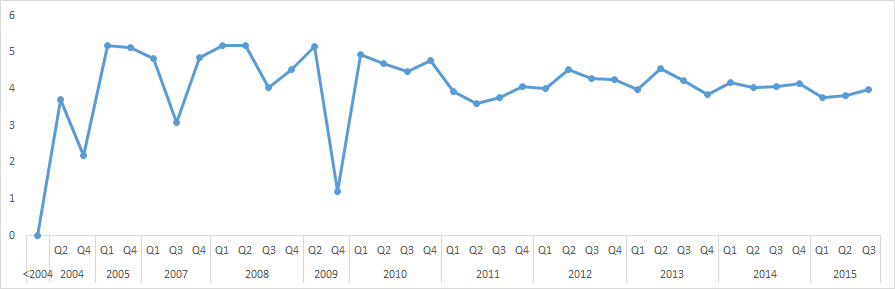
\includegraphics[width=15cm]{microwave.png}
  \caption{the R of microwave}
\end{figure}
\begin{figure}[h]
  \small
  \centering
  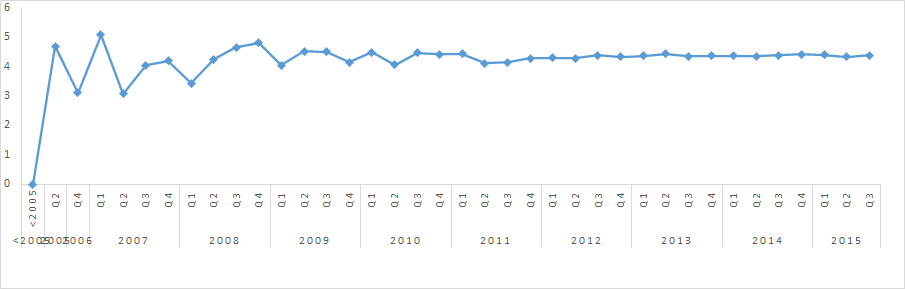
\includegraphics[width=15cm]{pacifier.png}
  \caption{the R of pacifier}
\end{figure}
\begin{figure}[h]
  \small
  \centering
  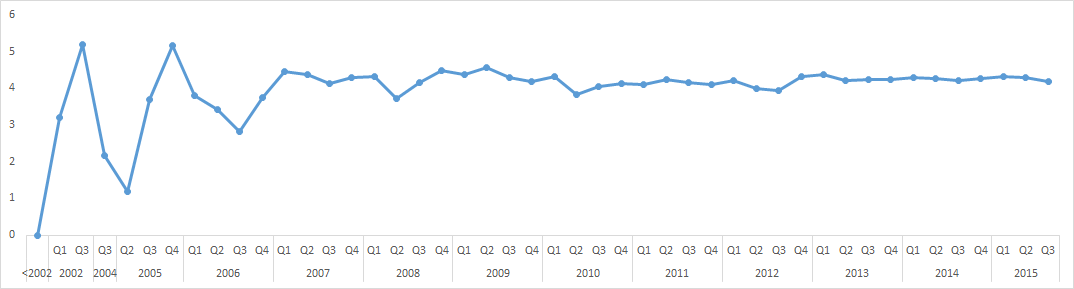
\includegraphics[width=15cm]{hair_dryer.png}
  \caption{the R of hair dryer}
\end{figure}

\subsection{descriptors of text based reviews \& rating levels}
We analyze the reviews of the three products by the LDA theme model. The extracted models are divided into five levels according to their emotional meanings, corresponding to 1-5 stars. For each review, the LDA model topic extraction is performed, and the corresponding star rating is calculated by weighting the topic proportion. The Pearson Correlation Coefficient between the star rating and the review score indicates correlation.

\begin{figure}[h]
  \small
  \centering
  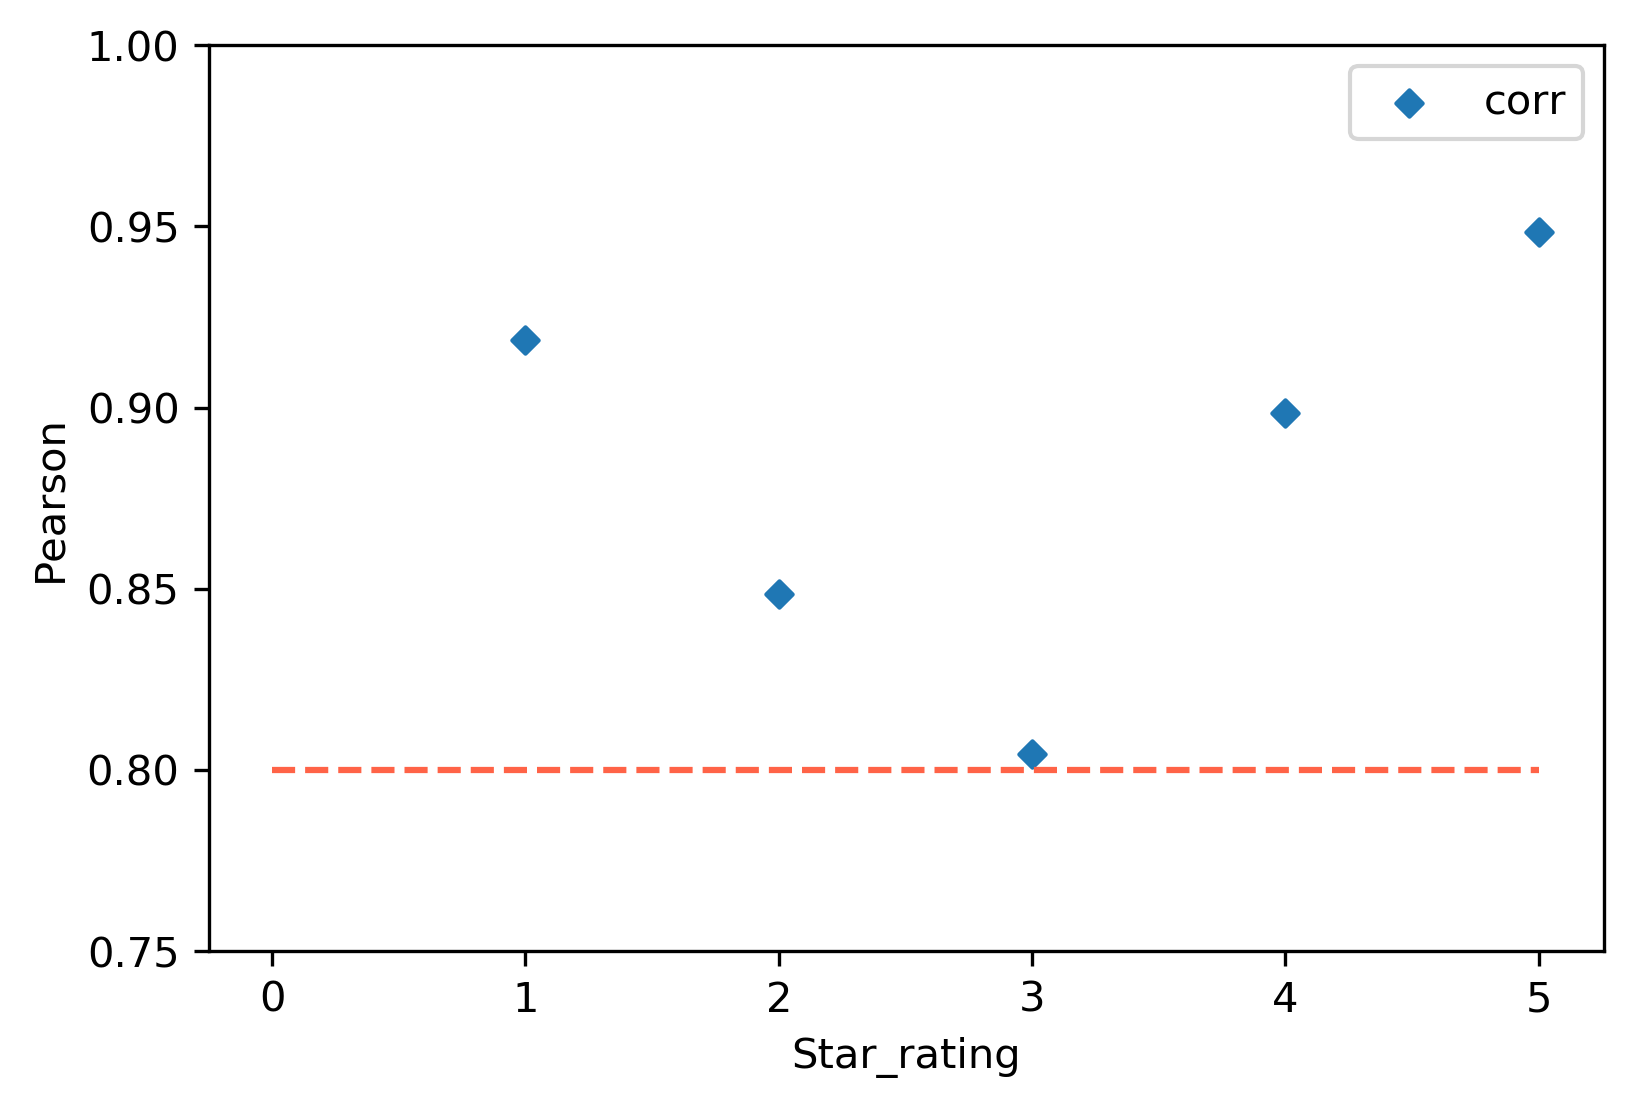
\includegraphics[width=12cm]{2e.png}
  \caption{correlation between rating and the review score}
\end{figure}

Illustrated by graphs, the correlation coefficient between each star rating and the review score exceeds 0.8, which shows that their similarity is high. However, it can be seen that the similarity of the 3 stars is the lowest among the whole, because the reviews are ambiguous, which leads to a great variation between the star and review semantic recognition scores.

\section{Strengths and Weaknesses}
\subsection{Strengths}
\begin{itemize}
  \item \textbf{Strong applicability}\\
   Our model can efficiently analyze reviews of various types of products, and the differences can be adapted by adjusting parameters.
  \item \textbf{Comprehensiveness}\\
  Various factors are considered in the assumptions and model design.
\end{itemize}

\subsection{Weaknesses and Improvement}
\begin{itemize}
  \item Due to the lack of sufficient data, the parameters used in the model are mainly obtained through actual life experience and repeated adjustment experiments. It would be profitable if we could get further data which can objectively reflect the quality of reviews or product quality, such as reviews with a more significant number of votes, or product sales data. By using these data, we are capable of performing a regression analysis on the model to obtain more accurate coefficients.
  \item The LDA model has an excellent performance with document collection, while the majority of reviews are short in words. 
  \item While major reviewers are not Amazon Vine Member, different people may have different criteria for evaluation, which may produce an objective assessment. We need to study every reviewers' rating habit to get a weight for every reviewer.
  \item Removing the non-purchasers' reviews helps analysis the problem; however, these overt reviews may hurt the customers' purchasing decisions and further ratings.
\end{itemize}

%% References
\begin{thebibliography}{99}
  \bibitem{1} Albert H. Huang, Kuanchin Chen, David C. Yen, Trang P. Tran,
  A study of factors that contribute to online review helpfulness,
  Computers in Human Behavior, Volume 48, 2015, Pages 17-27,
\end{thebibliography}

\end{document}

%% 
%% This work consists of these files mcmthesis.dtx,
%%                                   figures/ and
%%                                   code/,
%% and the derived files             mcmthesis.cls,
%%                                   mcmthesis-demo.tex,
%%                                   README,
%%                                   LICENSE,
%%                                   mcmthesis.pdf and
%%                                   mcmthesis-demo.pdf.
%%
%% End of file `mcmthesis-demo.tex'.
